\documentclass[a4paper, nofonts, nocap]{ctexart}

\usepackage[margin=1in]{geometry}
\usepackage{booktabs}
\usepackage{amsmath}
\usepackage{multirow}

\usepackage{listings}
\lstset{
	basicstyle=\ttfamily,
	tabsize=4,
	xleftmargin=2em,
	xrightmargin=1em,
	aboveskip=1em
}

\usepackage{fontspec}
\setmainfont{Times New Roman}
\setsansfont{Tahoma}
\setmonofont{Courier New}

\usepackage{xeCJK}
\setCJKmainfont[BoldFont={SimHei}, ItalicFont={KaiTi}]{SimSun}
\setCJKsansfont{SimHei}
\setCJKmonofont{FangSong}

\pagestyle{plain}

\renewcommand\figurename{图}
\renewcommand{\tablename}{表}

\begin{document}

\title{从豆瓣影评中提取电影标签 \\ \large ——中文信息处理课程项目}
\author{梁晓涛 \\ \small 13307130319}
\date{\today}
\maketitle

\tableofcontents
\newpage

\section{问题的背景}
在豆瓣的网站上对一部电影进行评价时,页面上会显示若干常用标签供用户参考(图 \ref{fig:douban})。并且每篇影评除了文章内容外,还有一个有用数和无用数(图 \ref{fig:useful}),表示其他用户赞同或反对这篇影评的数目,以及文章的发布时间等其他关于影评的数据。于是就想能不能利用这些数据,使用自然语言处理的技术,从用户的影评中自动提取电影的标签。
\begin{figure}[ht]
	\centering
	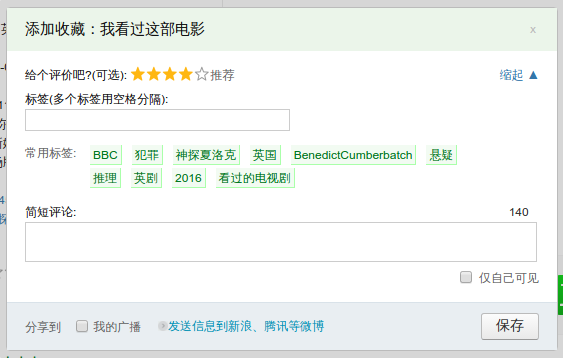
\includegraphics[width=0.9\textwidth]{images/douban.png}
	\caption{电影《神探夏洛克》的常用标签}
	\label{fig:douban}
\end{figure}

\begin{figure}[ht]
	\centering
	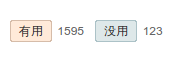
\includegraphics[scale=0.8]{images/useful.png}
	\caption{某篇影评的有用数和无用数}
	\label{fig:useful}
\end{figure}

\section{语料的收集和整理}
\subsection{爬取影评}
写了一个爬虫,自动以固定的频率从豆瓣上爬取电影下的长评,利用正则表达式从HTML页面中提取影评的数据,并把数据以CSV格式保存下来,每一行对应一篇影评(表 \ref{table:data},图 \ref{fig:data})。最终收集了20部电影的一共2000篇影评,CSV文件的总大小为8.4M。

\begin{table}[ht]
	\centering
	\begin{tabular}{llllllll}
		\toprule
		subject & movie & title & star & time & useful & useless & content \\
		\midrule
		电影在豆瓣的编号 & 电影名字 & 标题 & 评分 & 发布时间 & 有用数 & 无用数 & 文章内容 \\
		\bottomrule
	\end{tabular}
	\caption{数据描述}
	\label{table:data}
\end{table}

\begin{figure}[ht]
	\centering
	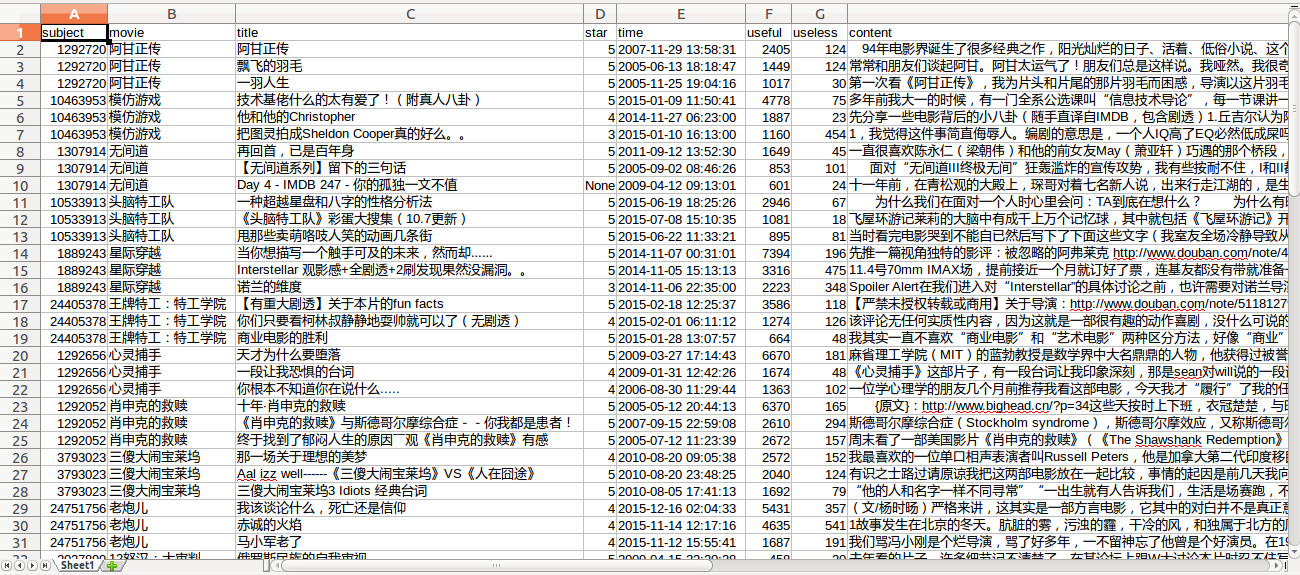
\includegraphics[width=\textwidth]{images/data.png}
	\caption{一小部分数据的截图}
	\label{fig:data}
\end{figure}

\subsection{处理文本}
\begin{enumerate}
	\item 把文章中的HTML标签去掉,只保留标签之间的内容
	\item 对文章分词\footnote{使用“结巴”中文分词 http://github.com/fxsjy/jieba}
	\item 只保留匹配\verb|[a-zA-Z0-9\u4E00-\u9FFF]+|的词,从而把中英文的标点符号和空白字符去掉
	\item 英文字母全部转为小写,以确保同一个单词不会因形式不同而被错认为是不同单词
	\item 利用中英文停用词表,将停用词去掉
\end{enumerate}

\section{关键词提取算法}
\subsection{TF-IDF}
TF-IDF是一种用于评估一个词对一个文档集中其中一份文档的重要性的统计方法,以下作简单介绍,具体可参考这篇文献\footnote{H.C. Wu, R.W.P Luk, K.F. Wong, K.L. Kwok "Interpreting TF-IDF term weights as making relevance decisions". \textit{ACM Transactions on Information Systems} 26(3):1-37, 2008.}。它的主要思想是:词频TF,表示一个词在一篇文档中出现的频率,如果该词在文档中频繁出现,则说明该词很好地代表了这篇文档的文本特征;逆向文件频率IDF,用来衡量一个词对文档的区分能力,如果文档集中包含这个词的文档越少,则说明这个词的类别区分能力越强,IDF也就越小。而TF-IDF将两者综合起来,词$w_i$对于文档$d_j$的权重为
\[ TFIDF_{i, j} = TF_{i, j} * IDF_i \]
\[ TF_{i, j} = \frac{n_{i, j}}{\sum_k n_{k, j}} \]
其中$n_{i, j}$表示词$w_i$在文档$d_j$中的出现次数,分母表示文档$d_j$中所有词的出现次数之和。
\[ IDF_i = \log \frac{|D|}{|{j:w_i \in d_j}|} \]
$|D|$表示文档集中的文档总数,$|\{j:w_i \in d_j\}|$表示包含词$w_i$的文档数目。

\subsection{基于TF-IDF的关键词提取算法}
对于从影评中提取关键词的问题,可以重新描述如下:

有$K$类文档$C_1, C_2, \dots, C_K$,$C_i$包含第$i$部电影的影评$d_{i, j}$,$C_i = \{d_{i, 1}, d_{i, 2}, \dots \}$,每篇文档$d_{i, j}$都有一个属性集$attr_{i, j}$,属性集中包含这篇影评的有用数、无用数、发布时间等数据。而我们的问题就是要给每类文档$C_i$提取关键词,要求关键词既能表示这类文档的文本特征,又能区分不同类别的文档。

一个简单的想法是,对于文档类$C_i$,直接把其中的文档$d_{i, j} \in C_i$合成一个文档$d_i$,文档集$D = \{d_1, d_2, \dots, d_K\}$,利用上节介绍的TF-IDF,求出合成文档$d_i$每个词的TF-IDF,取TF-IDF最大的若干个词作为$C_i$的关键词。

这个简单想法的主要问题是没有利用影评的属性信息。例如,对于同一类文档$C_i$,显然有用数多的文档比有用数少的文档更能表示$C_i$。于是,我们考虑通过修改TF-IDF来提取关键词,除了使用影评的文章内容外,还使用影评的属性数据,从而提高关键词的相关性。

具体的做法如下:

对于每一篇文档$d_{i, j}$,假设如果一个用户认为这篇文档有用,则相当于他写了一篇一模一样的文档,而如果一个用户认为这篇文档无用,则抵消一篇。如果无用数比有用数还多,则认为这篇文档对于表示$C_i$毫无贡献,所以计算文档$d_{i, j}$的得分为
\[ t_{i, j} = \max \{usefull_{i, j} - useless_{i, j} + 1, 0\} \]
利用每篇文档的得分$t_{i, j}$,计算词$w_l$在$C_i$内文档的词频的加权平均
\[ \overline{TF}_l^i = \frac{\sum_j t_{i, j}*TF_{l, j}^i}{\sum_j t_{i, j}} \]
其中$TF_{l, j}^i$表示词$w_l$在$d_{i, j}$中的词频。

IDF描述词$w_l$的区分能力,计算IDF的时候并不区分一个词属于哪一个文档类,即相当于把不同类别的文档组成一个文档集
\[ IDF_l = \log \frac{\sum_i |C_i|}{|\{(i, j):w_l \in d_{i, j}\}|} \]
其中分子表示包括不同类别的所有文档数,分母表示包含词$w_l$的文档数目。

于是词$w_l$对于文档类$C_i$的权重为
\[ TFIDF_l^i = \overline{TF}_l^i * IDF_l \]
取修改版TF-IDF最大的若干个词作为$C_i$的关键词。

\section{实验结果}
在语料库和对数据的预处理都相同的情况下,分别使用简单版TF-IDF (TF-IDF)和修改版TF-IDF (TF-IDF*)对选取的电影提取标签。表 \ref{table:label} 中显示了部分实验结果,其中每部电影包含三行标签,依次是豆瓣上的常用标签、TF-IDF提取的标签、TF-IDF*提取的标签,每行包含10个标签,并且后两行的标签按权重递减的顺序排列。
\begin{table}[ht]
	\centering
	\begin{tabular}{c|c}
		\toprule
		提取方式 & 标签\\
		\midrule
		& 12怒汉:大审判 12 \quad (2027899)\\
		豆瓣 & \verb|米哈尔科夫 俄罗斯 剧情 人性 俄罗斯电影 翻拍 Mikhalkov 2007 电影 法律| \\
		TF-IDF & \verb|法律 陪审团 男孩 俄罗斯 无罪 12 怒汉 车臣 有罪 审判| \\
		TF-IDF* & \verb|俄罗斯 车臣 美版 12 陪审团 战争 法律 男孩儿 男孩 案件| \\
		\midrule
		& 饮食男女 \quad (1291818)\\
		豆瓣 & \verb|台湾电影 张艾嘉 李安 饮食男女 家庭 剧情 台湾 伦理 中国 电影| \\
		TF-IDF & \verb|女儿 父亲 李安 闷骚 家庭 老朱 朱 朱师傅 同期 饮食男女| \\
		TF-IDF* & \verb|父亲 情结 埃勒克 特拉 女儿 家倩 一个 李安 朱师傅 艺术品| \\
		\midrule
		& 肖申克的救赎 \quad (1292052)\\
		豆瓣 & \verb|信念 剧情 人生 经典 美国 人性 自由 励志 1994 犯罪| \\
		TF-IDF & \verb|安迪 Andy 自由 监狱 瑞德 体制 肖申克 希望 Red 救赎| \\
		TF-IDF* & \verb|斯德哥尔摩 自由 安迪 Andy 监狱 体制 瑞德 习惯 Red 综合症| \\
		\midrule
		& 星际穿越 \quad (1889243)\\
		豆瓣 & \verb|宇宙 人性 美国 星际 冒险 亲情 2014 科幻 剧情 悬疑| \\
		TF-IDF & \verb|Cooper 黑洞 人类 诺兰 库珀 星际 洞 穿越 虫 星球| \\
		TF-IDF* & \verb|黑洞 Cooper Matthew 人类 洞 虫 诺兰 星球 女儿 地球| \\
		\midrule
		& 三傻大闹宝莱坞 \quad (3793023)\\
		豆瓣 & \verb|搞笑 剧情 励志 印度 人生 宝莱坞 喜剧 经典 爱情 2009| \\
		TF-IDF & \verb|na 印度 兰彻 Rancho 理工 电影 梦想 祖碧 杜比 学生| \\
		TF-IDF* & \verb|印度 Rancho na 途 兰彻 理工 病毒 兰乔 傻瓜 也许| \\
		\bottomrule
	\end{tabular}
	\caption{对比选取的标签}
	\label{table:label}
\end{table}

\subsection{豆瓣与TF-IDF*的标签的比较}
对于电影《12 怒汉:大审判 12》,豆瓣和TF-IDF*的公共标签有“俄罗斯”、“法律”,豆瓣的标签还有表示电影类型的“剧情”、“翻拍”,导演的中英文名字“米哈尔科夫”、“Mikhalkov”,以及跟具体电影无关的词“电影”。TF-IDF*则提取了几个特别的词“车臣”、“美版”、“战争”,“车臣”和“战争”反映了电影故事的背景是俄罗斯和车臣之间的战争,而“美版”反映了用户把这部翻拍的电影与1957年美版的电影进行比较。可以注意到TF-IDF*的标签中同时包含了“男孩儿”和“男孩”这两个表达相同含义的词。

对于电影《饮食男女》,豆瓣和TF-IDF*的公共标签有“李安”,豆瓣的标签还有表示电影类型的“剧情”、“伦理”,演员的名字“张艾嘉”。TF-IDF*则提取了几个特别的词“情结”、“埃勒克”、“特拉”、“父亲”、“女儿”,“埃勒克特拉情结”概括的是一种“恋父”情节,这几个词是对电影情节的更深层次的挖掘。但TF-IDF*的标签中也包含了“一个”等无用的词。

对于电影《星际穿越》,豆瓣的标签更多的是概括电影的剧情:“人性”、“冒险”、“亲情”、“科幻”、“剧情”、“悬疑”。TF-IDF*则提取了跟物理现象有关的词“黑洞”、“洞”、“虫”、“星球”、“地球”,这反映了很多影评在解释这些物理概念以帮助分析剧情。注意到“虫洞”一词被拆分成了两个词,这是分词的问题,但TF-IDF*还是能把“洞”和“虫”两个词排在一起。

总的来说,豆瓣的标签主要的用途是帮助用户给电影分类,所以往往出现导演名字、演员名字、电影的年份、电影的类型,以及一些概括电影剧情的词,同时还有一些用处不大的词,如“电影”。而TF-IDF*提取的词,如果包含了导演或演员的名字,往往是因为他们对这部电影贡献特别大或者表现特别突出。TF-IDF*能够提取一些表达电影更深层次的内涵的词,如电影的主题和背景。

\subsection{TF-IDF与TF-IDF*的标签的比较}
对于电影《饮食男女》,TF-IDF提取的词大部分只是一些在电影中频繁出现的词:“女儿”、“父亲”、“家庭”、“老朱”、“朱师傅”。而TF-IDF*则能提取出一些总结性、表示观众观点的词:“情结”、“埃勒克”、“特拉”、“艺术品”。并且可以注意到,TF-IDF提取的“朱”、“老朱”、“朱师傅”三个词都表示相同的意思,而TF-IDF*中的只出现了“朱师傅”。这主要是不同用户对同一个对象的叫法不同导致,而TF-IDF*相比简单TF-IDF更集中于某些影评,从而在一定程度上减少同义词的出现。

对于电影《三傻大闹宝莱坞》,“na”这个词在两种方法中都有出现。通过检查语料库,发现这个词之所以出现是因为有一篇影评引用了电影中的歌曲,歌词中大量出现“na”这个词,虽然“na”的IDF很小,但它的TF实在太大,导致总的权重大。但TF-IDF*并没有像简单TF-IDF那样把这个词排在了第一,只是排在了第三,说明TF-IDF*相比于简单TF-IDF更能降低“噪声”。

总的来说,简单TF-IDF倾向于提取电影中频繁出现的词,而TF-IDF*能提取表达观众观点的词,并且能相对地降低一些同义词、噪声词的权重。

\section{总结}
本项目提出了一个从豆瓣影评中提取电影标签的方法,该方法从经典的TF-IDF方法出发,利用影评的元数据得到了效果更好的关键词。相比于理论知识,在实际应用中需要考虑更多的东西:怎么获取语料库,怎么处理杂乱的数据,怎么利用实际应用中数据的各种信息改进理论的方法。

本项目还有许多可以改进的地方。提取的关键词的效果跟分词的效果直接相关,限于影评语料库的大小,分词时只利用了结巴分词的语料库,如果利用影评语料库来分词,是否可以更好地发现未登陆词,从而提高关键词的质量。提出的算法只基于简单的统计,相信如果考虑语义、词性等,能得到更好的效果。除了利用影评的有用数、无用数,还可以利用发布时间等其它信息,甚至可以把用户的账号信息利用起来。

\appendix

\section{代码的说明}
目录结构:
\begin{lstlisting}
	code/
	├── subject_list.txt			# 记录电影在豆瓣上的ID
	├── douban_big.csv			# 影评数据
	├── chinese_stopwords.txt		# 中文停止词
	├── scratch.py				# 爬虫
	└── extract.py				# 关键词提取
\end{lstlisting}

依赖:
\begin{itemize}
	\setlength{\itemindent}{2em}
	\item Python3 (http://www.python.org/)
	\item Jieba (http://github.com/fxsjy/jieba)
	\item NLTK (http://www.nltk.org/)
\end{itemize}

\subsection{scratch.py}
该脚本用于从豆瓣上爬取影评数据:
\begin{itemize}
	\setlength{\itemindent}{2em}
	\item 从文件 \verb|subject_list.txt|中读入需要爬取数据的电影的ID
	\item 为了防止被封IP,两次网络请求之间至少相隔1.5s
	\item 通过修改脚本中的 \verb|MaxLimit|变量,控制每部电影最多爬取的影评数目
	\item 爬取的数据保存在文件 \verb|douban.csv|中
\end{itemize}

使用命令:\verb|python3 scratch.py|

\subsection{extract.py}
该脚本用于从爬取的影评数据中提取关键词。

使用命令:
\begin{lstlisting}
	Usage: python3 extract.py [options] filename
	filename: 影评数据的文件名
	optinos:
		-k [NUM]:	指定提取关键词的数目,默认是10
		-w:			要求输出关键词的权重
\end{lstlisting}

\end{document}

